\chapterimage{Figures/laser.png} % Chapter heading image
% eLIGO laser copyright LIGO? AEI?

\chapter{Light Sources}
%\section{Light Sources}
\label{sec:Light_sources}
%{\color{blue} edited on 17 May by Benno\\
%	edited on 7 Aug by Benno\\
%edited on 5 Nov by Benno\\
%added IAP to Fig  21Nov\\
%edited 14 Jan 2019 by Benno}

This section describes 3G light sources, including the pre-stabilized high power lasers (PSLs) and the squeezed light sources. 
% Filter cavities for frequency dependent squeezing quadrature rotation are covered in the auxiliary optics chapter.

\section{Current State of the Art}
% \noindent{\bf High power lasers}
All currently operating advanced gravitational-wave detectors were designed to operate with a 200\,W class pre-stabilized laser system (PSL). All PSLs were independently developed following different approaches for the required high power lasers (HPL). A $ 200\,{\rm W} $ injection locked high power oscillator was installed at LIGO~\cite{Kwee:12}, a fiber based master oscillator power amplifier (MOPA) design was chosen for Virgo and KAGRA built on a MOPA design with fiber and solid-state amplifiers. Due to an unexpectedly high jitter noise coupling, Advanced LIGO is currently being operated with 70\,W MOPA systems using commercial solid-state amplifier (neoVAN 4S). A similar system with 100\,W power (neoVAN 4S-HP) was installed in Advanced Virgo as the tested 200\,W fiber MOPA solutions did not work reliably. KAGRA is currently operated with a 40\,W Nufern fiber amplifier. Commercial seed lasers (Mephisto series, Coherent) are being used in all PSL derivations. The high power stages are either built by industry or research labs. 

R\&D is globally underway towards a stable 200\,W light source with sufficiently low power noise, frequency noise and beam jitter. 
The ongoing R\&D in Nice, at MIT and in Hanover is devoted to reliability tests of 200\,W fiber amplifiers. A coherent combination of two 100\,W class solid-state amplifiers is being investigated in Hanover and a combination of two 40\,W class fiber amplifiers followed by a high power solid-state amplifier is tested in Japan. All of these high power laser operate at a wavelength of 1064\,nm and are of relevance for the 3G laser development at this wavelength. At $ 1.5\, {\rm \mu m}$ and in the $ 2\, {\rm \mu m}$ region, high power laser R\&D toward developing concepts for 3G detectors is being performed in Adelaide, IIT Madras, Hamburg and Hanover. HPLs with approximately 100\,W output power have or will soon be demonstrated by these groups. 
% inside the gravitational-wave community. 

Other HPL developments that were not specifically tailored for gravitational-wave applications can be found in the literature. These designs often fall short of one or more of the stringent requirements for 3G high power light sources. To the best of our knowledge, there is no commercially available HPL with the specifications required for 3G. A market survey should be carried out to substantiate this statement.

Non-classical light sources at 1064\,nm generating up to 15\,dB of squeezed vacuum have been developed for the currently operating advanced GWDs. These sources have reached maturity, as shown by GEO600's several years of operation with squeezed light and the use of squeezing in Advanced LIGO and Advanced Virgo. Squeezed light sources at $ 1.5\, {\rm \mu m}$ have reached similar squeezing levels but no system design efforts were undertaken yet to transfer the laboratory systems to prototypes. At $ 2\, {\rm \mu m}$ a few dB of squeezing were demonstrated recently in a laboratory experiment at ANU.

%{\bf High power lasers demonstrated in lab}\\
%{\color{red}to be filled}
%\begin{itemize}
%	\item 1064\,nm
%	\item 1550\,nm
%	\item $\rm 2\,\mu m m$ (taken from M. Steinke GWADW2018 talk)\\
%	\begin{tabular}{|c|c|c|c|c|}
%		\hline 
%		\textbf{power} & \textbf{linewidth} & \textbf{M2} & \textbf{remark} & \textbf{reference} \\ 
%		\hline 
%		600\,W & $< 10\,MHz$ & 1.05 & non-monolithic & [1] \\ 
%		\hline 
%		200\,W &$ <2\,MHz$ & 1.6 & monolithic, PER 17\,dB & [2] \\ 
%		\hline 
%		300\,W & $<100\,kHz$ &  & few modes $\rm 25\mu m m fiber $ & [3] \\ 
%		\hline 
%	\end{tabular} \\
%\end{itemize}
% $[1]$ Goodno et al., Opt. Lett. 34 (8)\\
% $[2]$ Liu et al, Opt. Express 22\\
% $[3]$ Wang et al, IEEE Photon. Technol. Lett. 27 (6)\\
%
%{\bf squeezed light sources demonstrated in lab}	
%\begin{itemize}
%	\item 1064\,nm
%	\item 1550\,nm
%	\item $\rm 2\,\mu m m$
%\end{itemize}
%

\section{Requirements and current/planned R\&D}
%To evaluate the R\&D currently performed within the worldwide gravitational wave (GW) community a questionnaire was send to 32 laser and squeezing experts in all GW projects. The questionnaire asked for current and planned R\&D and for desired collaboration topics and coordination mechanisms. We found, that the current or planned research of at least two groups cover all the identified required research areas (see Fig.\ref{fig:LightSourceRD}) 
%The current or planned research of at least two groups cover all the identified required research areas (see Fig.\ref{fig:LightSourceRD}) 

%\magentacomment{hal: Include pointer to a living document instead of static table? Suggested by GWIC 3G committee}

%\begin{figure}[ht]
	% \centering
%	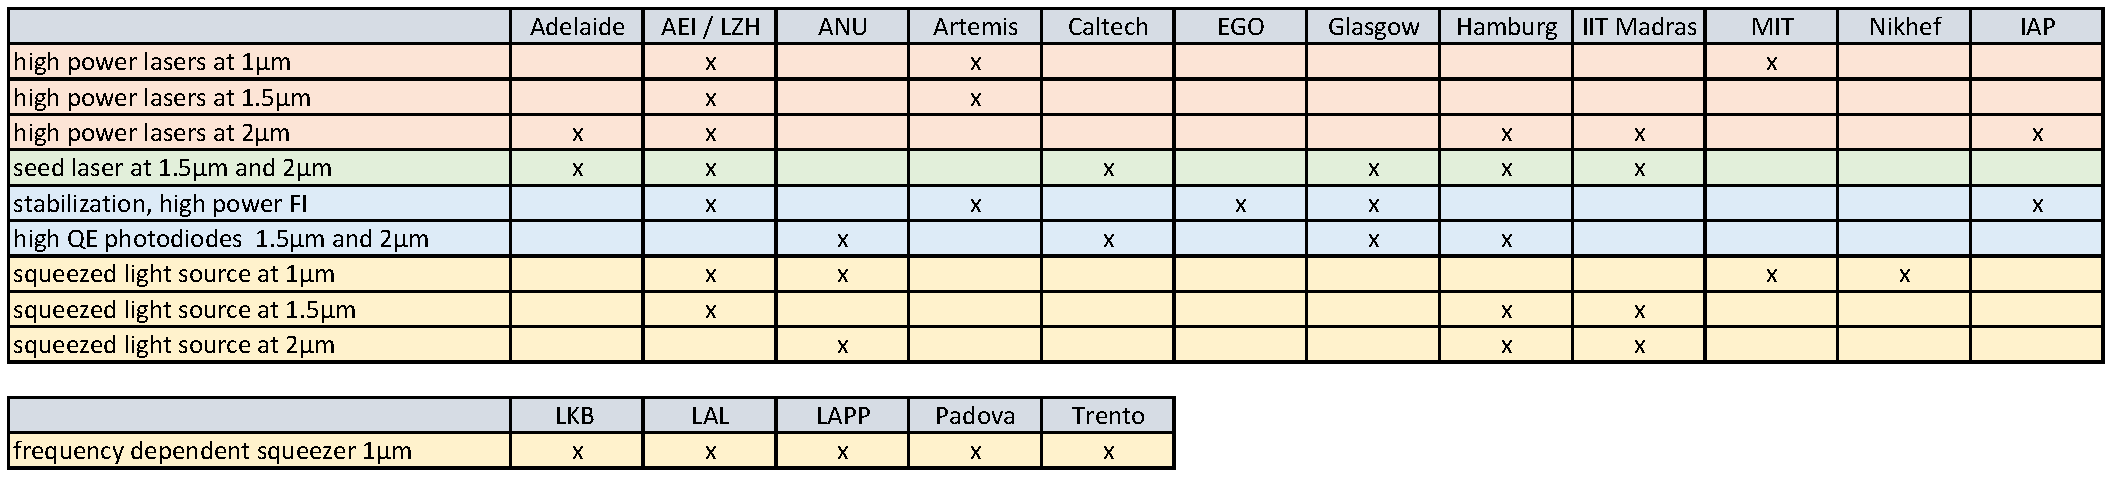
\includegraphics[width=\textwidth]{Figures/Light_source_Fig1.png}
%	\caption{Current or planned R\&D on high power laser and squeezed vacuum sources}
%	\label{fig:LightSourceRD}
%\end{figure}

A survey within the gravitational-wave community showed that more than 10 groups currently perform R\&D on light sources for 3G detectors. All relevant research topic are being worked on by at least two groups. A snapshot of which group is working on which topic can be found at~\cite{LightSource_RD_table}. We also analyzed available documentation and presentations on 3G detectors to extract requirements for the high power lasers and squeezers.

The requirements for the PSL and the squeezed light sources for 3rd generation detectors are not yet well defined. The Einstein Telescope~\cite{ET2011} builds on a 500\,W laser at 1064\,nm in the spatial $\rm LG_{33}$ mode and a 3\,W laser at a wavelength of 1550\,nm in the fundamental Gaussian mode.
% \greencomment{Dave: It might be good to include a simple summary table of the current knowledge of the requirements for laser performance for ET, CE, and Voyager} \magentacomment{hal: there is some space left at the end of the chapter, so space-wise we could} 
Even though these are clear requirements, the ET design is currently being reevaluated. In particular the operation of the ET high power IFO in the spatial $\rm LG_{33}$ seems questionable. The current  LIGO Voyager design is built on a HPL with a power of 200\,W and a wavelength of 1550\,nm or longer for absorption by Silicon test masses. Cosmic Explorer~\cite{CosmicExplorer2017} will require a HPL within the same wavelength interval but with much higher power. This power level is currently not well defined but may be as high as 1\,kW~\cite{GWADW2018,ISWP:2018}. The wavelength choice depends on several factors, such as the availability of high power lasers, absorption of the substrates and the high reflective coatings of the test masses, scattering and the availability of photo detectors with high quantum efficiency. As information on several of these factors is missing, a final wavelength choice can not yet be made. Currently wavelengths of 1550\,nm and around $\rm 2\, \mu m $ and $\rm 2.1\, \mu m $ are favored due to promising high power laser concepts for these wavelengths. Hence R\&D on HPL for three different wavelengths (1064\,nm, 1550\,nm and around $\rm 2\, \mu m $) has to be performed until the final wavelengths are selected. 
No information on PSLs stability requirements for 3G detectors exists at present. As a 10 times better sensitivity is aimed for we assume that the power, frequency and beam jitter stability has to be a factor of 10 higher than in advanced detector PSLs. Concerning the spatial and polarization purity we expect similar requirements as for the advanced detectors.
All 3G detector designs currently incorporate 10\,dB of detected squeezing, meaning that squeezed vacuum sources with squeezing levels of $> 15\,dB$ are required.

Thus, in this report we assume that \emph{initially} 250\,W at 1064\,nm and 500\,W at  $ 1.5\, {\rm \mu m}$ or in the $ 2\, {\rm \mu m}$ region will be required. We expect that a factor of 10 less noise compared to 2G PSLs and similar spatial and polarization purity as in 2G PSLs will be needed. Furthermore, we assume that a squeezing level of 15\,dB will be sufficient for \emph{initial} 3G detector operation. For the \emph{final} 3G detectors, we expect that  500\,W at 1064\,nm and 1\,kW at  $ 1.5\, {\rm \mu m}$ or in the $ 2\, {\rm \mu m}$ region again with similar stability and beam purities as in the initial 3G phase will be required. A \emph{final} squeezing level requirement of 20\,dB is assumed.

%\begin{itemize}
%	\item HPL with a power of 250\,W at 1064\,nm with a factor of 10 less noise compared to the 2G PSL and similar spatial and polarization purity requirements as 2G PSLs
%	\item HPL with a power of 500\,W at  $ 1.5\, {\rm \mu m}$ or in the $ 2\, {\rm \mu m}$ region with a factor of 10 less noise compared to the 2G PSL and similar spatial and polarization purity requirements
%	\item Squeezed light sources at all three wavelength with 15\,dB squeezing level
%\end{itemize}
%
%For the final 3G GWD configurations the following PSL requirement are assumed:
%\begin{itemize}
%	\item HPL with a power of 500\,W at 1064\,nm with stability and purity as above
%	\item HPL with a power of 1\,kW at  $ 1.5\, {\rm \mu m}$ or in the $ 2\, {\rm \mu m}$ with stability and purity as above
%	\item Squeezed light sources at all three wavelength with 20\,dB squeezing level
%\end{itemize}


\section{Pathways and required facilities} \label{sec:pathway}
The pathway towards adequate PSLs for 3G detectors has several steps:
\begin{enumerate}
	\item Demonstration of reliable high power generation with required power level, low enough free-running noise (defined by stabilization constraints) and acceptable spatial and polarization purity (functional prototype)
	\item Design, fabrication and test of a HPL according to reproducible fabrication steps with the required diagnostic and stabilization actuators. Demonstration of long-term stable operation and conceptual demonstration of the stabilization concept (engineering prototype).
	\item Final design steps as part of a 3G project and reliability test of the stabilization concept.
\end{enumerate}

\noindent Item 1 is part of generic laser research and is typically performed by university or laser research laboratories. We expect, that up to a power level of $ \approx 200 \, {\rm W} $ this research will be done in the laboratories listed in \cite{LightSource_RD_table}, but new groups may also join the effort. Together with a coherent combination step this work should be sufficient for the 1064\,nm 3G HPL development.
A new coordinated R\&D effort is required to develop a 1\,kW class laser with a wavelength longer than or equal to $ 1.5\, {\rm \mu m}$.
% {\color{red} @Benno: Do we have any idea on how to generate 1\,kW in one step? Or do we need to combine 4 x 250\,W lasers?}
% Benno's answer: No I don't

The reliability and reproducibility part of the engineering step needs a dedicated program of a large laser research lab or industrial involvement. The scope of this step is normally not included in the programs of research funding agencies, so a dedicated R\&D funding program will be required to cover the costs.
Furthermore specific infrastructure and trained staff is required for the fabrication part of the engineering prototype phase. The assembly and stabilization part can be done in one of the laboratories of the GWD community (see \cite{LightSource_RD_table}) or in newly joining laser labs. The same holds true for one or several coherent combination steps. Depending on the progress of the wavelength decision, the engineering prototype step needs to be conducted for two or three wavelengths. During this phase several identical HPLs should be built and characterized in a long term test.

The final design step is part of each specific 3G project and should be performed at an early stage of the respective project with project funding.

The pathway towards an adequate squeezed light source will most likely involve university and research lab based R\&D. The required funding is on a scale that can be covered by regular research grants and the development and improvement of non-classical light sources falls in standard calls of funding agencies. Squeezing levels of $ \approx 15 \, {\rm dB} $ have already been achieved for  $ 1\, {\rm \mu m}$ and  $ 1.5\, {\rm \mu m}$ such that the main technical challenges for these wavelengths are the reduction of loss in optical components and improving the stability and controllability of the squeezing phase. The squeezing research at $ 2\, {\rm \mu m}$ is far less advanced and substantial effort has to be put into the generation of high squeezing levels and low loss components. Several parallel efforts should continue for each wavelength as this approach allows to compare different technical solutions and chose the most appropriate for each project when project funding arrives.

%\subsubsection{functional prototypes}
%Show that high power generation concepts works reliable, accept poor noise performance, missing diagnostic and actuators for stabilization
%\subsubsection*{1064\,nm}
%we assume reliability problem of 200\,W class fiber amplifier will be solved for Advanced detectors (current work at AEI/LZH, MIT and Artemis)\\
%develop coherent combination techniques at 2x250\,W power level
%\subsubsection*{1550\,nm}
%assume AEI/LZH fiber amplifier development is successful
%\subsubsection*{$\rm \bf 2\,\mu m m$}
%assume either Adelaide cryo HM or wavelength doubling of 1064\,nm in OPA is successful
%\subsubsection*{stabilization}
%develop stabilization concepts for all three wavelength adequate for free running noise and available actuators of functional PT developments
%\subsubsection{engineering prototype}
%after final wavelength selection transfer concepts to laser lab or company capable of designing and fabricating an engineering prototype that meets all requirements concerning power, noise performance, spatial and polarization purity, actuators with sufficient range and bandwidth, diagnostic\\
%transfer engineering prototype to research lab for characterization and pre-stabilization\\
%build several engineering prototypes for long-term/reliability tests

\section{Type of collaboration required:  small/large}
Like in the past a strong collaboration between a group within the gravitational-wave community and a laser research lab or industry is required (such as AEI/LZH, Artemis/Alphanov, ICRR/Mitsubishi) to design and build suitable HPLs at the different wavelengths. As the different wavelengths need different solutions, a loose collaboration between the respective wavelength groups would be sufficient. It would be desirable to have at least two collaborations to work on laboratory prototype solutions for each wavelength to explore different concepts and alternative technical solutions. These groups should have a strong connection with regular meetings to exchange results and ideas. This approach would possibly avoid a single supplier problem.
No particular collaborations are required for the squeezing research. The normal exchange of concepts and results at collaboration meetings and conferences seems sufficient. 

\section{Road map}
\subsection*{HPL 1064\,nm}
\begin{itemize}
	\item 2019 - 2020 : continue development and reliability studies of 2G PSL systems at the 250\, W level and perform coherent combination demonstration experiments at high powers
	\item 2021 - 2024 : engineering prototype (see section \ref{sec:pathway}) 500\,W HPL and conceptual test of stabilization and spatial filter solutions
	\item 2024 - ... : final design and fabrication of HPL with the initial 3G requirements within specific 3G projects, in parallel R\&D on path toward the final 3G requirements 
\end{itemize} 


\subsection*{HPL ${\bf 1.5 - 2.1 \, {\bf \mu m}}$}
\begin{itemize}
	\item 2019 - 2021 : identify concepts for a 1\,kW HPL that fulfills the stringent 3G detector HPL requirements (most likely several coherently combined stages)
	\item 2022 - 2024 : 1\,kW HPL functional prototype phase (see section \ref{sec:pathway})
	\item 2024 - 2028 : 1\,kW HPL engineering prototype phase (see section \ref{sec:pathway})
	\item 2028 - ... : final design and fabrication of HPL with the initial 3G requirements within specific 3G projects, in parallel R\&D on path toward the final 3G requirements
\end{itemize} 


\subsection*{squeezed light sources for 3G GWDs}
\begin{itemize}
	\item 2019 - 2026 : continue laboratory based R\&D on squeezed light sources at all wavelength, potentially involve industrial partners to design and fabricate low loss optical components
	\item 2026 - ... : final design and fabrication within specific 3G GWD project
\end{itemize}

%\subsection{HPL 1064\,nm}
%\begin{tabular}{|p{1.8 cm}|p{10cm}|}
%	\hline 
%	\textbf{time} & \textbf{work}  \\ 
%	\hline 
%	2019-2020 &continue development and reliability studies of 2G PSL systems at the 250\, W
% level and perform coherent combination demonstration experiments at high powers \\ 
%	\hline 
%	2021-2024 & engineering prototype (see section \ref{sec:pathway} ) 500\,W HPL and conceptual test of stabilization and spatial filter solutions \\ 
%	\hline 
%	2024 - & final design and fabrication of HPL with the initial 3G requirements within specific 3G GWD project, in parallel R\&D on path toward the final 3G requirements \\ 
%	\hline 
%\end{tabular} \\

%\subsection{{HPL ${\bf 1.5 - 2.1 \, {\bf \mu m}}$}}
%\begin{tabular}{|p{1.8 cm}|p{10cm}|}
%	\hline 
%	\textbf{time} & \textbf{work}  \\ 
%	\hline 
%	2019-2021 &identify concepts for a 1\,kW HPL that fulfills the stringent 3G GWD HPL requirements (most likely several coherently combined stages)\\ 
%	\hline 
%	2022-2024 & 1\,kW HPL functional prototype phase (see section \ref{sec:pathway} ) \\ 
%	\hline 
%	2024 - 2028 & 1\,kW HPL engineering prototype phase (see section \ref{sec:pathway} ) \\ %
%	\hline 
%	2028 - & final design and fabrication of HPL with the initial 3G requirements within specific 3G GWD project, in parallel R\&D on path toward the final 3G requirements \\
%	\hline
%\end{tabular} \\

%\subsection{squeezed light sources for 3G GWDs}
%\begin{tabular}{|p{1.8 cm}|p{10cm}|}
%	\hline 
%	\textbf{time} & \textbf{work}  \\ 
%	\hline 
%	2019-2026 &continue laboratory based R\&D on squeezed light sources at all wavelength, potentially involve industrial partners to design and fabricate low loss optical components\\ 
%	\hline 
%	2026 - & final design and fabrication within specific 3G GWD project \\
%	\hline
%\end{tabular} \\

%\subsection{Suggested mechanisms}
%annual meetings, keep list of who does what,\\
%team up of GWD projects and funding agencies in engineering PT stage
%\subsection{Impact/relation to 2G and upgrades}
%at 1064\,nm laser development for 2G and upgrades is in direct path to 3G and will serve as long-term test of some concepts

%\subsection{Suggested mechanisms}
%annual meetings, keep list of who does what,\\
%team up of GWD projects and funding agencies in engineering PT stage
%\subsection{Impact/relation to 2G and upgrades}
%at 1064nm laser development for 2G and upgrades is in direct path to 3G and will serve as long-term test of some concepts